\begin{figure}
  \begin{subfigure}{0.4\textwidth}
    \[
    \text{IOU} = \frac{\text{Area of Intersection}}{\text{Area of Union}}
    \]
  \end{subfigure}%
  \begin{subfigure}{0.2\textwidth}
    \centering
    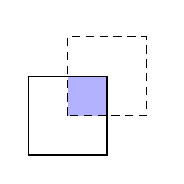
\begin{tikzpicture}
      \fill[color=blue!30] (0.5, 0.5) rectangle (1, 1);
      \node[draw=none] () at (1.5, 1.5) {};
      \draw (0, 0) rectangle (1, 1);
      \draw[densely dashed] (0.5, 0.5) rectangle (1.5, 1.5);
    \end{tikzpicture}
    \caption{IOU=0.14}
  \end{subfigure}%
  \begin{subfigure}{0.2\textwidth}
    \centering
    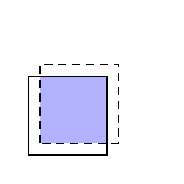
\begin{tikzpicture}
      \fill[color=blue!30] (0.15, 0.15) rectangle (1, 1);
      \node[draw=none] () at (1.5, 1.5) {};
      \draw (0, 0) rectangle (1, 1);
      \draw[densely dashed] (0.15, 0.15) rectangle (1.15, 1.15);
    \end{tikzpicture}
    \caption{IOU=0.57}
  \end{subfigure}%
  \begin{subfigure}{0.2\textwidth}
    \centering
    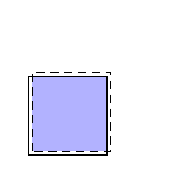
\begin{tikzpicture}
      \fill[color=blue!30] (0.05, 0.05) rectangle (1, 1);
      \node[draw=none] () at (1.5, 1.5) {};
      \draw[densely dashed] (0.05, 0.05) rectangle (1.05, 1.05);
      \draw (0, 0) rectangle (1, 1);
    \end{tikzpicture}
    \caption{IOU=0.82}
  \end{subfigure}
  \caption{Intersection over Union (IOU) illustration.}
  \label{fig:iou}
\end{figure}

%%% Local Variables:
%%% mode: latex
%%% TeX-master: "../network"
%%% End:
